%\linenumbers*
\chapter{EFFECT OF TEMPORAL RESOLUTION OF STORM DATA ON SOIL EROSION}
\label{sec:EFFECTSOFTEMPORALSCALESOFSTROMDATA}

\section{Introduction}
\label{sec:TemporalScalesEffectsIntroduction}

%******start with little bit of rationalization of this set of experiments and
%why did I choose to do THIS and why IN THIS WAY
When modelling soil erosion, finding suitable input data for the simulation is
an important part of model-based researches but it is not easy. Ideally, input
data need to be measured directly from a study site and parametrized for a model
simulation. However, this process requires a great effort and time. It is also
frequently affected by geographical and financial situations of research. All
these reasons affect how rainfall data are made available in different
resolutions
either spatially, temporally or both. Thus, we often end up using what is
readily available rather than what is really required by erosion models.

Rainfall intensity is highly variable depending on data resolutions and where
they
are measured from \citep{nyssen2005-172}. Consequently, using rainfall data
that have a undesired data resolution for erosion simulations may produce
unknown
implications that may later lead to inaccurate model outputs. Therefore, this
chapter aims to investigate effects of different temporal resolutions of
rainfall
data on erosion model simulation processes. In addition, which data format
between CLIGEN and breakpoint data is more suitable for current research was
looked at.

The results of this chapter and the subsequent chapters attempts to provide some
answers for Research Question \ref{researchquestion2}:\
\begin{quotation}
Assuming that we use a model to predict erosion rates under the future climate
which may have different rainfall intensities from the present, what information
do we need to make predictions in terms of both climate and process
understanding?
\end{quotation}

\section{Data Preparation and Method}
\label{sec:TemporalScalesEffectsMethods}

Two storms that occurred on 4 July 2000 and on 11 October 2000 were selected
from Plumpton event rainfall dataset (P) (Table
\ref{tab:DetailsOfDataStations}). The storm on 11 October 2000 was selected
because the rainfall amount of this event was exceptionally high (133.8 mm) for
the area and was related to severe erosion and property damage
\citep{boardman2001-346}. The return period for such a event is estimated at
around 300 years \citep{saunders2001-360}. All three stations that record event
rainfalls in the region observed a exceptional rainfall on the same day (Figure
\ref{fig:obs_daily_amount}). However, Plumpton station (P) recorded the highest
rainfall amount. This ``October'' storm was typical of frontal, low-intensity
event that occur in winters in South Downs, UK. In comparison, the ``July''
storm that occurred on 4 July 2000 was selected from the same year in order to
increase the diversity of storm patterns that are investigated in this chapter.
This storm is typical of summer storm that has a shorter duration than
``October'' storm (Table \ref{tab:DetailsoftworainstormsobservedinPlumpton}) and
has a distinctive high intensity peak in the middle of storm duration. Rainfall
amount of this storm also is comparably high and distinctive.

The duration of ``October'' event was 1208 minutes (i.e.\ 20 hours and 8
minutes). Average intensity for this rainfall was 6.65 mm/hr with 1-min peak
intensity of 84 mm/hr. The ``July'' rainfall, on the other hand, was recorded
with total rainfall amount of 74.8 mm and duration of 808 minutes (i.e.\ 13
hours and 28 minutes). Average intensity for this event was 5.5 mm/hr with
1-min peak intensity reaching to 60 mm/hr. The details of two events are
summarised in Table \ref{tab:DetailsoftworainstormsobservedinPlumpton}.

\begin{table}[htbp]
  \figureversion{tabular}
  \centering
  \small
  \caption{Details of two rain storms observed in Plumpton}
  \label{tab:DetailsoftworainstormsobservedinPlumpton}
    \begin{tabular}{lcc}
    \toprule
     & 11 October 2000 & 4 July 2000 \\
    \midrule
    Amount (mm) & 133.8 & 74.8\\
    Total duration (min) & 1208 & 808 \\
    Average intensity (mm/hr) & 6.7 & 5.5 \\
    Effective duration (min) & 460 & 313 \\
    1-min peak intensity (mm/hr) & 84 & 60 \\
    \bottomrule
    \end{tabular}
\end{table}

Tipping-bucket data for both events were aggregated into 5 different temporal
resolutions---1, 5, 15, 30 and 60 minutes. This was done to simulate different
temporal rainfall data resolution. Each temporal resolution was treated as if it
was the
``baseline'' resolution for the data with these being the only records
available. Two
sets of temporally varying ``July'' and ``October'' storm data were prepared
into CLIGEN and breakpoint data format for erosion estimations.

CLIGEN rainfall data describe a rainfall storm with four parameters: total
rainfall amount ($R$, inch), effective rainfall duration ($D$, minute),
normalised time to peak ($t_p$) and normalised peak intensity ($i_p$). Effective
daily rainfall duration was calculated by summing the number of temporal bins
with rainfall on the event day, after removing temporal bins without rainfall.
Effects of removing these ``gaps'' are investigated in the following section,
Chapter \ref{sec:EFFECTSOFCONTINOUSANDDISCONTINUSSTORM}. Normalised time to
peak is a relative time of peak intensity after the removal of gaps.
Normalised peak intensity is a peak intensity that is relative to average
rainfall intensity of the storm. These four parameters were calculated
individually for each temporal data resolution (Table
\ref{tab:CLIGENWEPPInputFileParameters}), and weather inputs for WEPP were
built (cf. Appendix \ref{sec:WEPPInputData}).

Breakpoint data, on the other hand, consist of two parameters: (accumulated)
rainfall time and (accumulated) rainfall amounts or intensity. Each dataset was
converted into these two parameters, and the number of breakpoints was counted.
Breakpoint weather inputs for WEPP are also shown in Appendix
\ref{sec:WEPPInputData}.

Then, two process-based erosion models, WEPP and EUROSEM, are used at the
current stage to simulate runoff and soil loss. RillGrow is not used here
because of the data resolution and computational time issues involved
with using RillGrow. Temporal resolutions that RillGrow simulates with is very
small
so that it requires a considerably long computational time compared to the
duration that is simulated for. To give an idea, RillGrow2 requires almost 7
hours, for example, for running a 45-min simulation. This makes using RillGrow
for this set of investigations very impractical considering the number of
simulations and the total duration of computational time required. Thus, only
two models, WEPP and EUROSEM, are used in this chapter.

CLIGEN data and breakpoint data prepared from rainfall data with 1, 5, 15,
30 and 60-min temporal resolution were used for the simulations to investigate
the
effect of different temporal resolution.
EUROSEM was designed to use only breakpoint rainfall data so that it would
be a good comparison to WEPP which has been originally designed to use CLIGEN
data as well as breakpoint data.
%why was RillGrow not used?? -- explained in the later chapter (chapter 6)

As pointed out, EUROSEM uses breakpoint rainfall data only. This means that,
unless the EUROSEM code was rewritten, using CLIGEN data directly with EUROSEM
is not possible. Rewriting of EUROSEM code would not be viable for the scope of
this research. Thus, to use CLIGEN data for EUROSEM simulations, an additional
procedure was carried out to make sure that the same rainfall data were used as
for WEPP simulations.

According to WEPP model document, WEPP disaggregates CLIGEN data into ten
breakpoints using a double exponential equation before calculating erosion
related parameters \citep[see][\S 2.2]{flanagan1995-usda}. These disaggregated
breakpoint data can be found in one of WEPP output files. For EUROSEM
simulations, these breakpoint data from WEPP outputs were used in place of
CLIGEN data. This makes the rainfall data used for WEPP and EUROSEM essentially
the same for both simulations (Figure \ref{fig:eurosem_cligen_workaround}).

\begin{figure}[htbp]
  \centering
    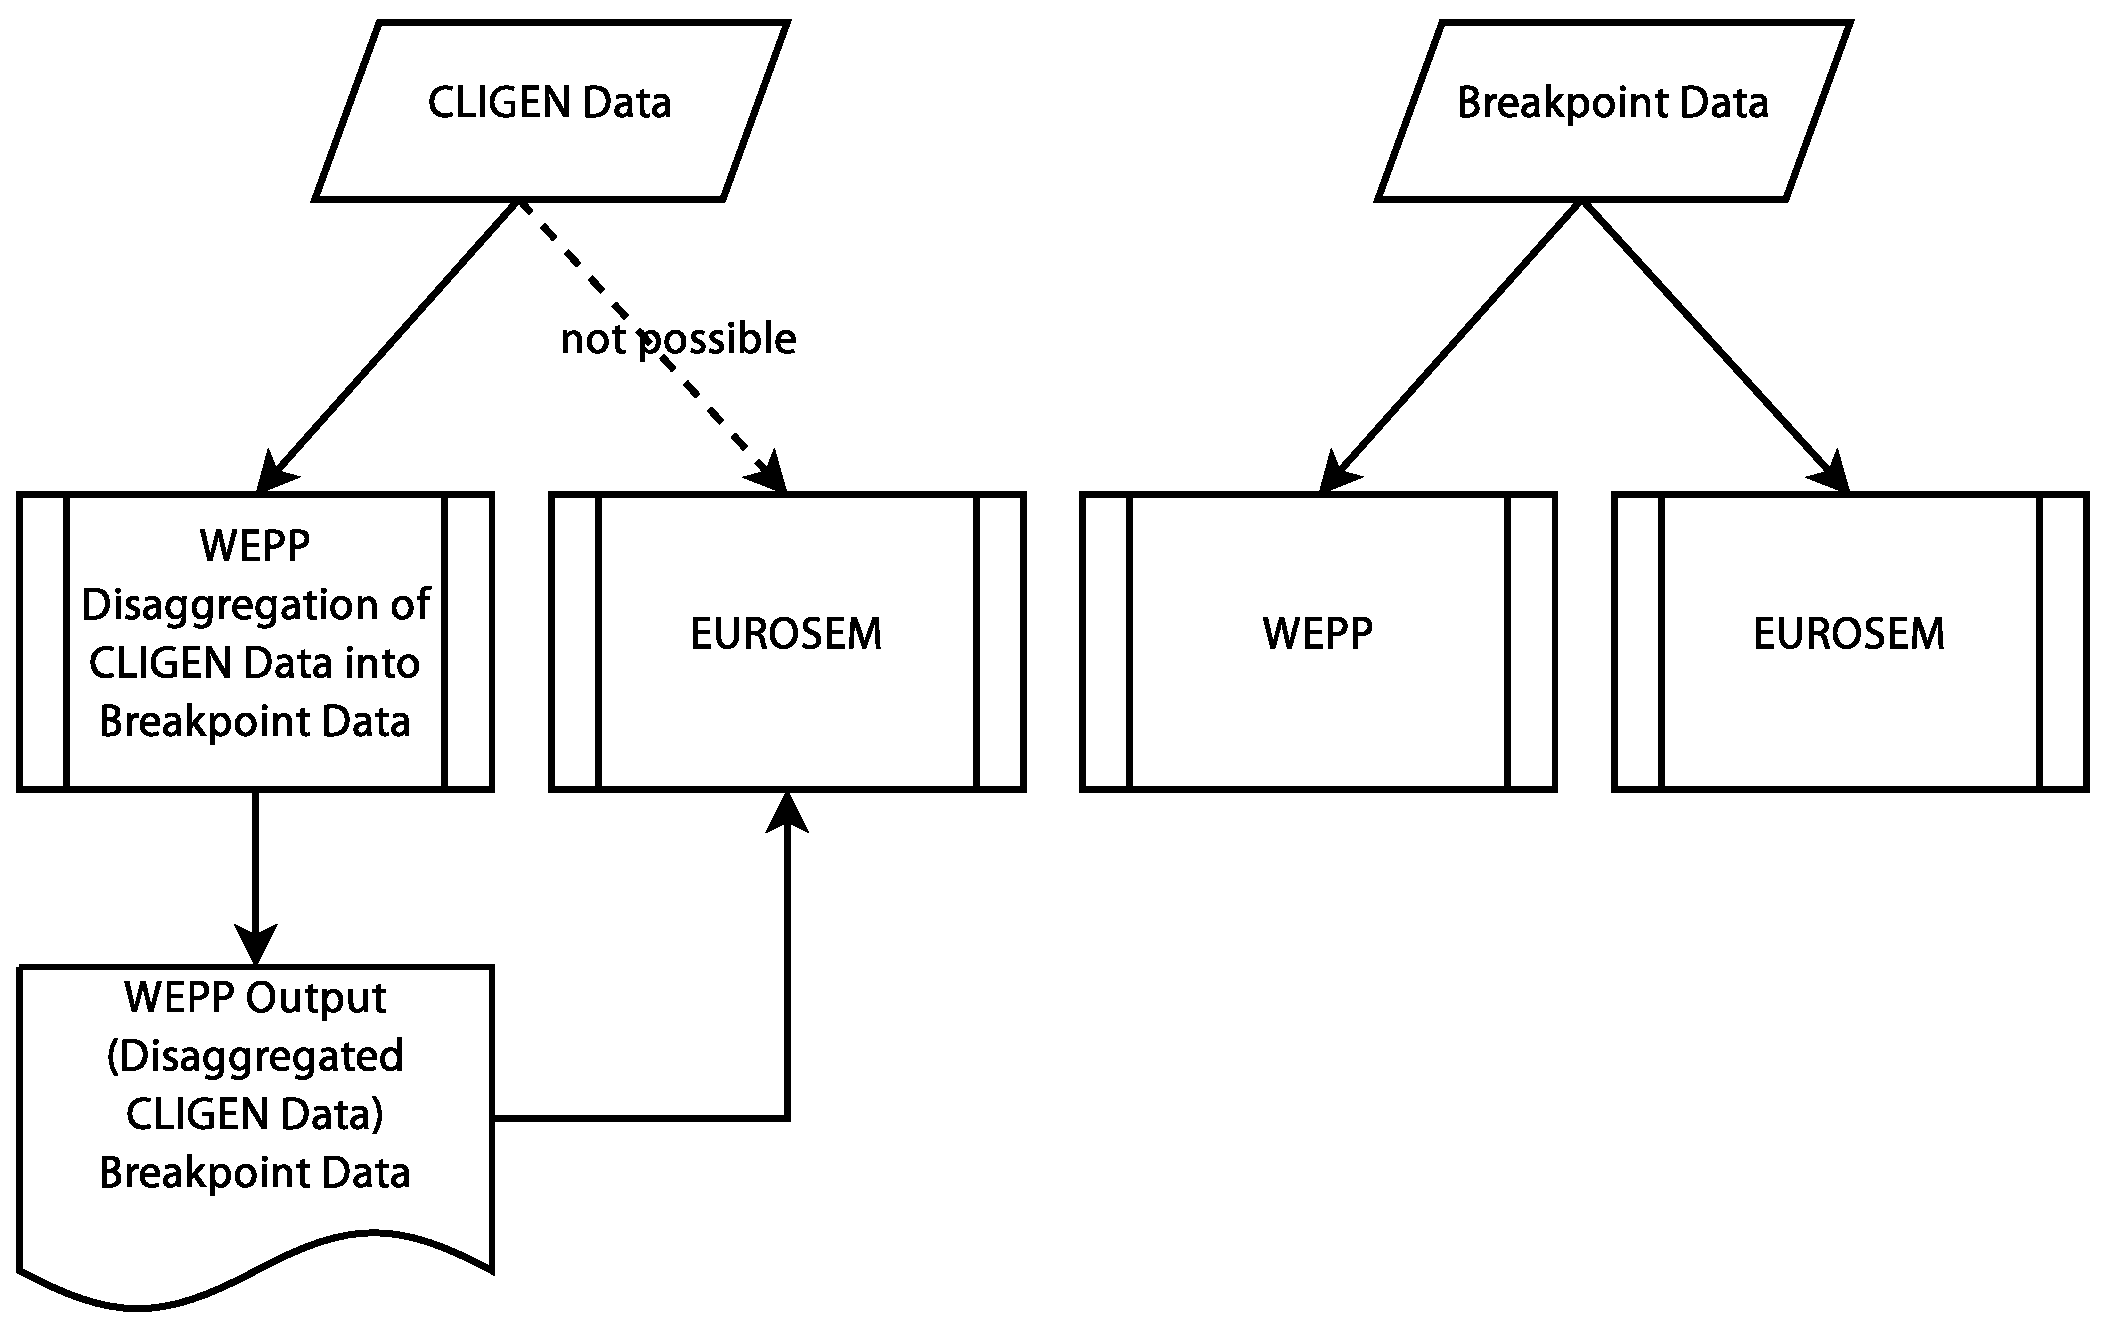
\includegraphics[width=0.8\textwidth]{./img/eurosem_cligen_workaround}
  \caption{A diagram of WEPP and EUROSEM simulations with CLIGEN and breakpoint
data}
  \label{fig:eurosem_cligen_workaround}
\end{figure}

Other inputs for EUROSEM were adopted from WEPP outputs as no direct
measurements were available to build EUROSEM inputs from scratch. This approach
may be problematic for certain modelling studies. However, in this research, it
permits a workaround to problems of unavailable factors for EUROSEM simulation.
It needs to be noted again that the emphasis of this research is not on
assessing the performance of models against measured data.

The effect of the temporal resolutions on rainfall intensity, runoff and soil
loss
were examined. For comparison purpose, 15-min data were used as a reference
resolution when comparisons were done to highlight the effects. 15-min
resolution is
the resolution that were used for the CLIGEN development.

%It may be a good idea to compare, or at least, talk  about little bit about
%the effects caused by using CLIGEN data or breakpoint data. By using one or
%another, are the effects enhanced or subdued for individual time resolutions,
%and also for overall?

\section{Effect on Rainfall Intensity Information}
\label{sec:EffectsOnRainfallIntensityInput}

CLIGEN data for two storms were built by calculating rainfall amount, duration,
peak intensity and time to peak. These values were individually calculated for
each temporal resolution. The details of the input parameters are shown in Table
\ref{tab:CLIGENWEPPInputFileParameters}.

\begin{table}[htbp]
  \figureversion{tabular}
  \centering
  \small
  \caption{CLIGEN data parameters for two rain storms observed in
Plumpton}
  \label{tab:CLIGENWEPPInputFileParameters}
    \begin{tabular}{rcccccccc} \toprule
       & \multicolumn{4}{c}{11 October 2000} &
\multicolumn{4}{c}{4 July 2000}\\
       \cmidrule(r){2-5} \cmidrule(l){6-9}
       & amount & duration$^{\dagger}$ & $t_p$ & $i_p$ & amount &
duration$^{\dagger}$ & $t_p$ & $i_p$\\
       %\addlinespace[-1mm]
       & \scriptsize(mm) & \scriptsize(hr) & & & \scriptsize(mm) &
\scriptsize(hr) & & \\
       \midrule
      1-min  & 133.8 & 7.4  & 0.12 & 4.64 & 74.8 & 5.2  & 0.63 & 4.20\\
      5-min  & 133.8 & 12.8 & 0.46 & 5.53 & 74.8 & 11.1 & 0.58 & 6.41\\
      15-min & 133.8 & 15.5 & 0.49 & 2.87 & 74.8 & 13.3 & 0.54 & 3.69\\
      30-min & 133.8 & 17   & 0.93 & 2.69 & 74.8 & 14   & 0.52 & 2.95\\
      60-min & 133.8 & 18   & 0.64 & 2.23 & 74.8 & 14   & 0.54 & 2.65\\
      \bottomrule
      %\addlinespace[1mm]
      \multicolumn{9}{l}{\footnotesize $^\dagger$ effective rainfall
duration, {\normalsize{$t_p$}}: normalised time-to-peak, {\normalsize{$i_p$}}:
normalised peak intensity}
    \end{tabular}
\end{table}

As shown is Table \ref{tab:CLIGENWEPPInputFileParameters}, each set of
temporally varying rainfall data shows different total rainfall durations. This
is because of their time intervals being in different sizes. Therefore,
effective rainfall duration increases as temporal data resolution increases.
With
rainfall amounts remaining the same, the changes in duration mean that rainfall
intensity information is also affected by the temporal resolution of rainfall
data.
Peak rainfall intensities are affected by the data resolution too. Moreover, the
change of temporal resolution shifts the temporal location of peak intensity
($t_p$). This means that the shape of a storm may change from, for example,
ascending intensity to descending intensity. Effects of storm shapes on soil
erosion are further investigated in Chapter
\ref{sec:EFFECTSOFRAINFALLINTENSITYCHANGESONSOILEROSION}.

\begin{table}[htbp]
  \figureversion{tabular}
  \centering
  \small
  \caption{Number of time intervals (breakpoints) for each temporal resolution}
  \label{tab:maxnooftimeintervalsperday}
    \begin{tabular}{lccccc}
    \toprule
    Temporal resolution (min) & 1 & 5 & 15 & 30 & 60 \\ \midrule
    4 July 2000 & 315 & 135 & 55 & 30 & 16 \\
    11 October 2000 & 460 & 152 & 63 & 35 & 19 \\
    Max. no. of intervals (per day) & 1440 & 288 & 96 & 48 & 24 \\
    \bottomrule
    \end{tabular}
\end{table}

For breakpoint data, the maximum numbers of time intervals per day as well as
the number of breakpoints for each storm are shown in Figure
\ref{tab:maxnooftimeintervalsperday}. The number of breakpoints for the storms
decreases as the temporal resolution increases. Also, the rainfall data with
different temporal resolutions show different rainfall intensity information
(Figure
\ref{fig:dr_storm} and \ref{fig:pl_storm}). Higher temporal resolution data show
higher instantaneous peak rainfall intensities. With 1-min data of the
``October'' storm, for example, a peak rainfall intensity was over 80 mm/hr
(Figure \ref{fig:pl_storm-a}). In comparison, 60-min data of the ``October''
storm show no peak rainfall intensity higher than 20 mm/hr (Figure
\ref{fig:pl_storm-e}). This is because rainfall intensity is averaged over the
length of each time step. Time to peak rainfall intensity is also different for
each temporal resolution depending on which two bins (i.e.\ breakpoints) added
together and averaged (Figure \ref{fig:dr_storm} and \ref{fig:pl_storm}).

\begin{figure}[htbp]
  \centering
  % These are called DR storm but in fact they are Plumpton July storm
    \subfloat[]{\label{fig:dr_storm-a}
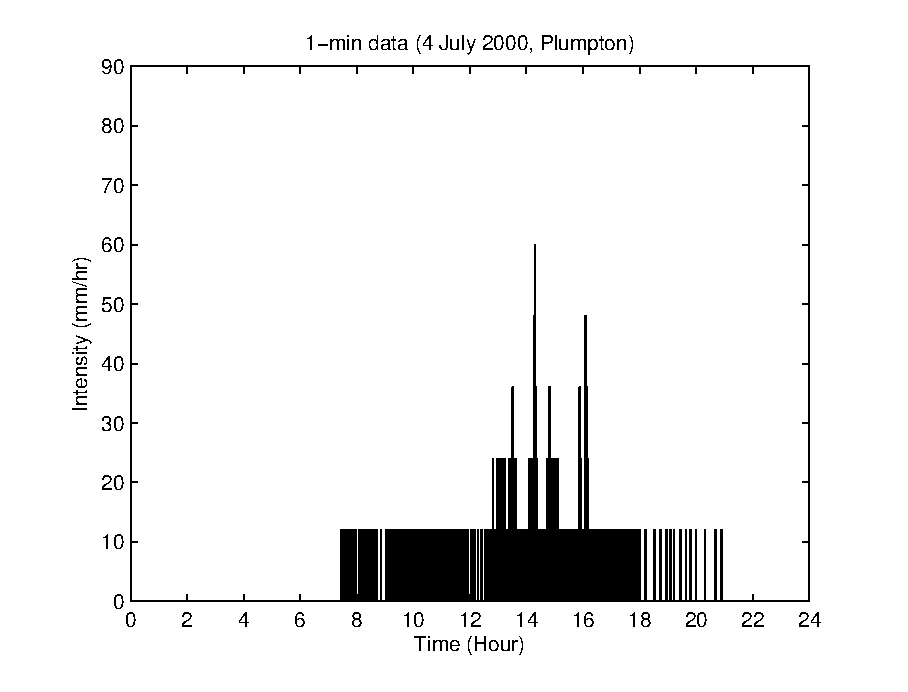
\includegraphics[width=0.49\textwidth]{./img/dr_storm_1min}}
    \subfloat[]{\label{fig:dr_storm-b}
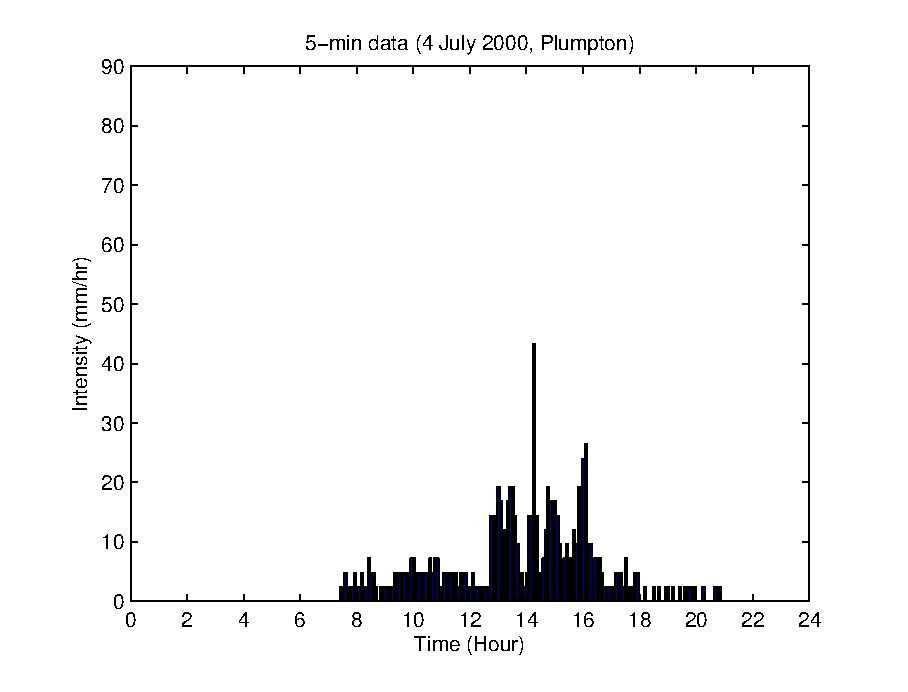
\includegraphics[width=0.49\textwidth]{./img/dr_storm_5min}}
    \qquad
    \subfloat[]{\label{fig:dr_storm-c}
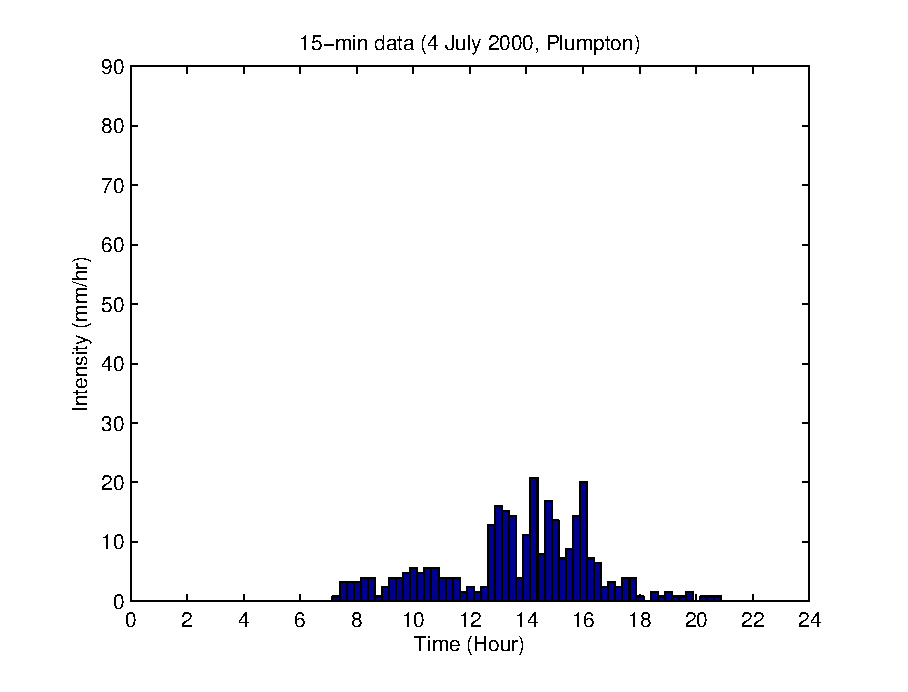
\includegraphics[width=0.5\textwidth]{./img/dr_storm_15min}}
    \qquad
    \subfloat[]{\label{fig:dr_storm-d}
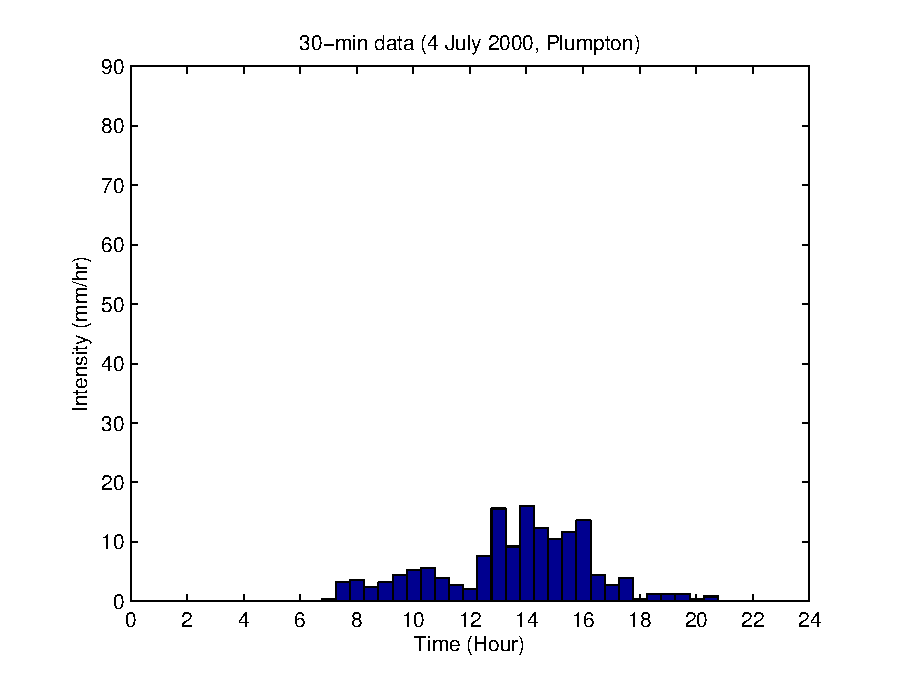
\includegraphics[width=0.49\textwidth]{./img/dr_storm_30min}}
    \subfloat[]{\label{fig:dr_storm-e}
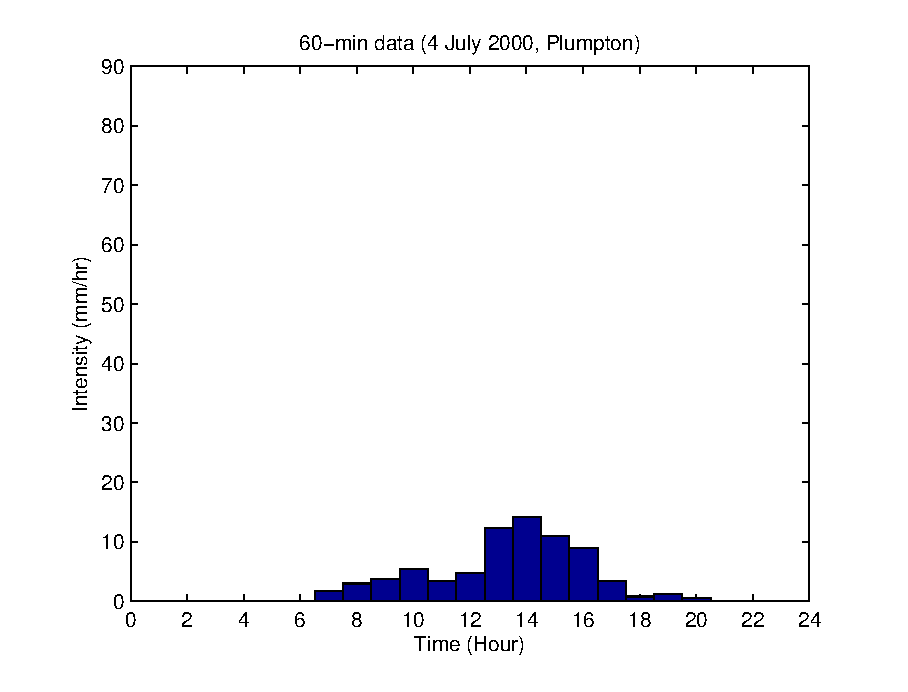
\includegraphics[width=0.49\textwidth]{./img/dr_storm_60min}}
  \caption{Various temporal resolutions of original breakpoint data for 4 July
2000
storm in Plumpton}
  \label{fig:dr_storm}
\end{figure}

\begin{figure}[htbp]
  \centering
    \subfloat[]{\label{fig:pl_storm-a}
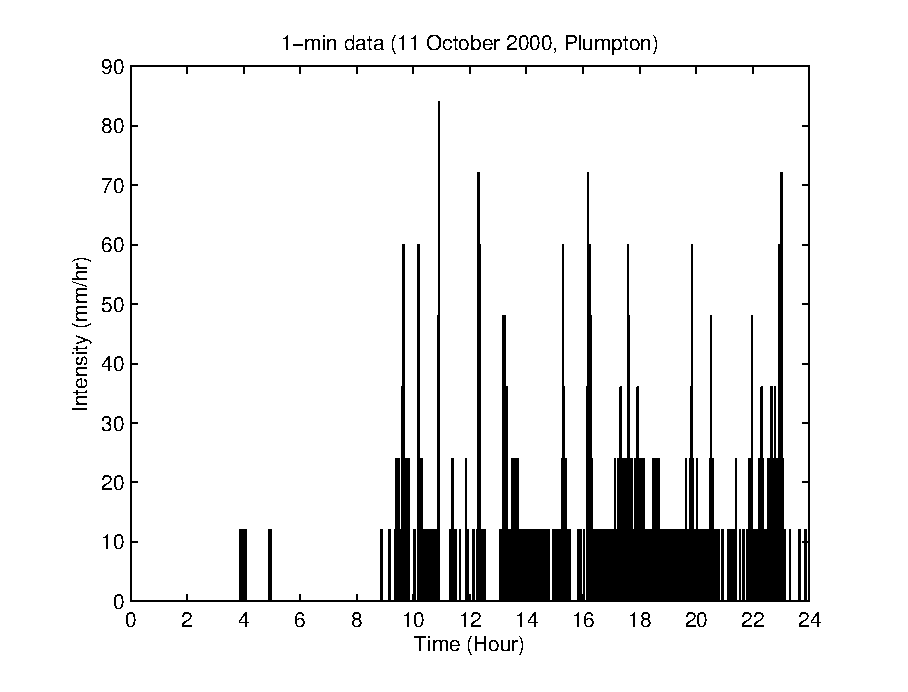
\includegraphics[width=0.49\textwidth]{./img/pl_storm_1min}}
    \subfloat[]{\label{fig:pl_storm-b}
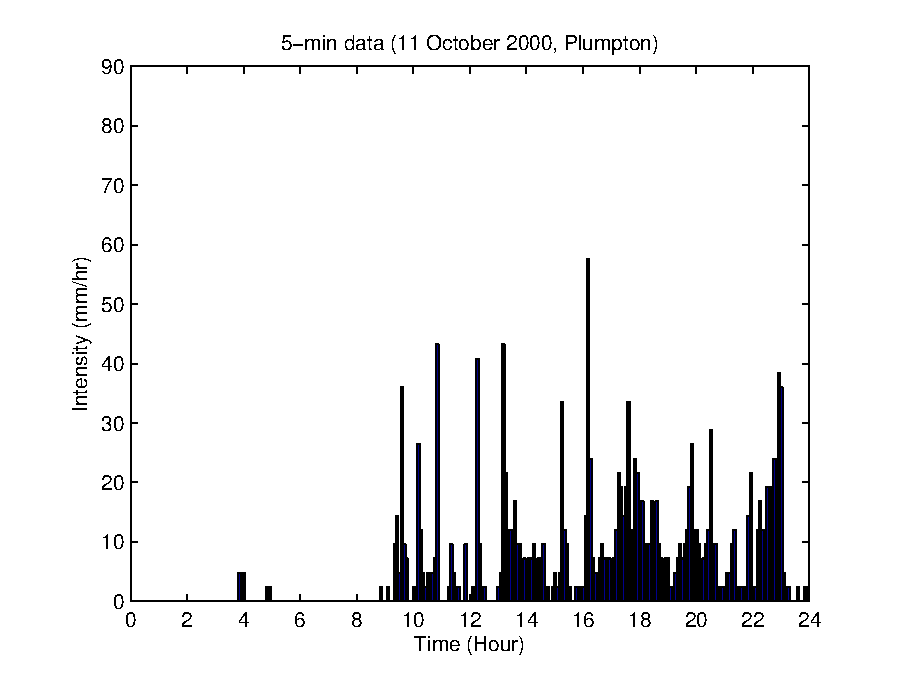
\includegraphics[width=0.49\textwidth]{./img/pl_storm_5min}}
    \qquad
    \subfloat[]{\label{fig:pl_storm-c}
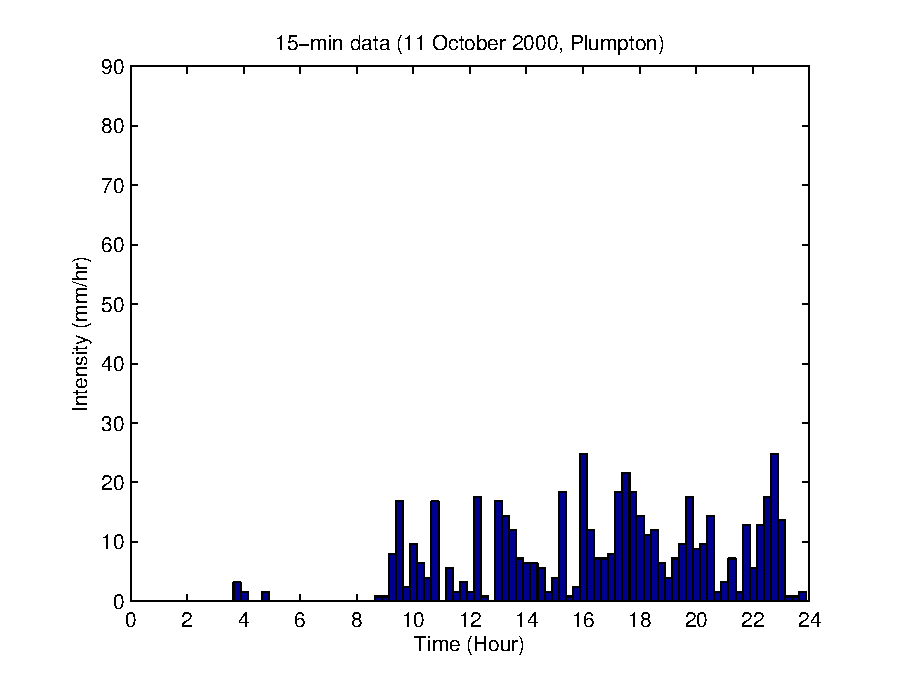
\includegraphics[width=0.5\textwidth]{./img/pl_storm_15min}}
    \qquad
    \subfloat[]{\label{fig:pl_storm-d}
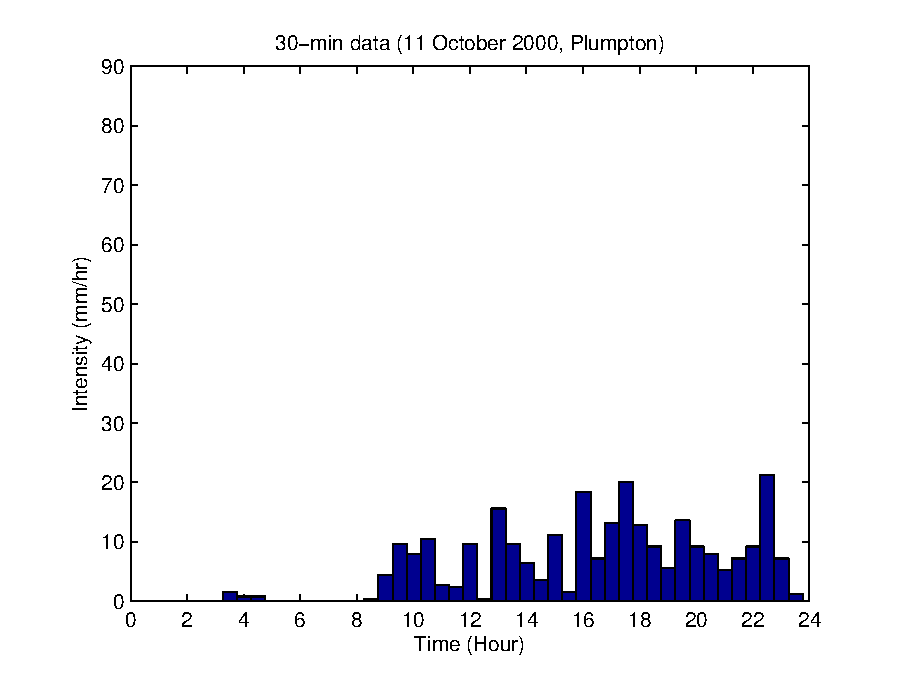
\includegraphics[width=0.49\textwidth]{./img/pl_storm_30min}}
    \subfloat[]{\label{fig:pl_storm-e}
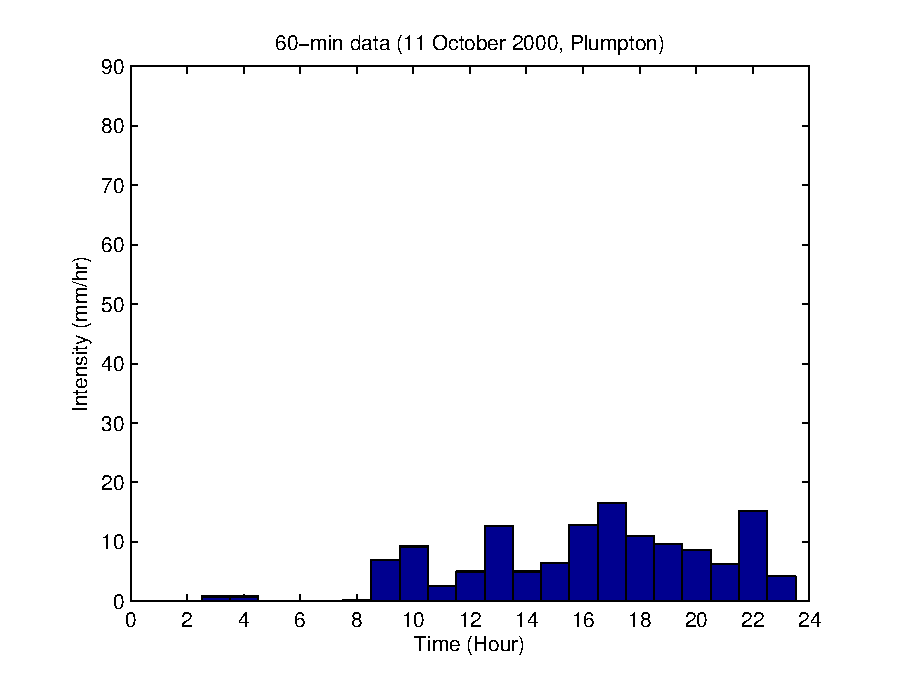
\includegraphics[width=0.49\textwidth]{./img/pl_storm_60min}}
  \caption{Various temporal resolutions of original breakpoint data for 11
October
2000 storm in Plumpton}
  \label{fig:pl_storm}
\end{figure}

\section{Effect on Simulated Runoff and Soil Loss}
\label{sec:TemporalScalesSimulatedRunoffAndSoilLoss}

The breakpoint data prepared for both ``October'' and ``July'' events with 1 and
5-min time intervals could not be used for WEPP and EUROSEM because of model
limitations. During investigation, it was found that WEPP and EUROSEM limits the
total number of breakpoints that they can process
\citep{flanagan1995-weppusersummary, morgan1998-europeansoilerosion}. These
limitations are discussed further later in the chapter. Thus, no runoff and soil
loss rates were estimated with 1 and 5-min breakpoint data. Instead, CLIGEN data
with 1 to 60-min resolutions and breakpoint data with 15 to 60-min resolutions
were used
to estimate runoff and soil loss rates.

\subsection{Effect of Temporal resolution on Runoff}
\label{sec:TemporalScalesSimulatedRunoff}

In overall, WEPP and EUROSEM estimated greater runoff when rainfall data
with high temporal resolutions were used than when rainfall data with low
temporal
resolutions were used. However, this is only true for CLIGEN data type. For
breakpoint data format, the effect of temporal data resolutions is rather
unclear for
both models.
%You need to be more specific about what you are trying to say here. --
%getting more specific as I build up the argument.

Runoff amounts estimated by WEPP with CLIGEN and breakpoint rainfall data for
each temporal resolution are shown in Table
\ref{tab:DifferentTemporalScalesOfRainfallDataOnWEPPRunoffEstimation}. Results
from WEPP simulations show that the changes of runoff rates from the runoff
rates simulated with 15-min CLIGEN data are greater when simulated with 1-min
CLIGEN data than with 5-min CLIGEN data. For example, using 1-min data instead
of 15-min data of ``July'' storm resulted in about 45\% increase in runoff and
30\% increases for ``October'' storm (Table
\ref{tab:DifferentTemporalScalesOfRainfallDataOnWEPPRunoffEstimation}). Using
60-min data, on the other hand, of the same storms results in about 20\% and
10\% decreases in runoff amounts compared to using 15-min data, respectively
(Table \ref{tab:DifferentTemporalScalesOfRainfallDataOnWEPPRunoffEstimation}).
The effect of changes of temporal resolutions are greater when CLIGEN data of
the
July event are used than the October event.

\begin{table}[htbp]
  \figureversion{tabular}
  \centering
  \footnotesize
  \caption[WEPP-estimated runoff with different temporal resolutions of CLIGEN
and
breakpoint rainfall data]{WEPP-estimated runoff (mm) with different temporal
resolutions of CLIGEN and breakpoint rainfall data}
  \label{tab:DifferentTemporalScalesOfRainfallDataOnWEPPRunoffEstimation}
    \begin{tabular}{lllllll}
      \toprule
      & & \multicolumn{5}{c}{Temporal Resolution}\\
      \cmidrule{3-7}
      Data type & Event & 1-min & 5-min & 15-min & 30-min & 60-min \\
      \midrule
      CLIGEN & 4 Jul 2000 & 49.7 ($+$44.5) & 44.5 ($+$29.4) & 34.4 & 29.3
($-$14.8) & 27.0 ($-$21.5) \\
       & 11 Oct 2000 & 97.4 ($+$29.9) & 89.4 ($+$19.2) & 75.0 & 75.0 & 67.5
($-$10.0) \\
       \midrule
      Breakpoint & 4 Jul 2000 & $-$ & $-$ & 30.4 & 29.8 ($-$2.0) & 29.7
($-$2.3)\\
       & 11 Oct 2000 & $-$ & $-$ & 63.9 & 68.5 ($+$7.2) & 69.9 ($+$9.4)\\
      \bottomrule
      %\addlinespace[1mm]
      \multicolumn{7}{p{12cm}}{\footnotesize Figures in (\ ) are the \% changes
from the result with the 15-min data. $+/-$ indicates a increase or decrease.}\\
    \end{tabular}
\end{table}

\begin{table}[htbp]
  \figureversion{tabular}
  \centering
  \footnotesize
  \caption[EUROSEM-estimated runoff (mm) with different temporal resolutions of
CLIGEN and breakpoint rainfall data]{EUROSEM-estimated runoff (mm) with
different temporal resolutions of CLIGEN and breakpoint rainfall data}
\label{tab:DifferentTemporalScalesOfRainfallDataOnEUROSEMRunoffEstimation}
    \begin{tabular}{lllllll}
      \toprule
      & & \multicolumn{5}{c}{Temporal Resolution}\\
      \cmidrule{3-7}
      Data type & Event & 1-min & 5-min & 15-min & 30-min & 60-min \\
      \midrule
      CLIGEN & 4 Jul 2000 & 53.3 ($+$54.1) & 42.2 ($+$22.0) & 34.6 & 31.5
($-$9.0) & 30.7 ($-$11.3) \\
       & 11 Oct 2000 & 102.1 ($+$22.6) & 93.6 ($+$12.4) & 83.3 & 80.1 ($-$3.8) &
75.9 ($-$8.9) \\
       \midrule
      Breakpoint & 4 Jul 2000 & $-$ & $-$ & 33.2 & 32.6 ($-$1.8) & 37.0
($+$11.5) \\
       & 11 Oct 2000 & $-$ & $-$ & 62.7 & 69.1 ($+$10.2) & 74.4 ($+$18.7)\\
      \bottomrule
      %\addlinespace[1mm]
      \multicolumn{7}{p{12cm}}{\footnotesize Figures in (\ ) are the \% changes
from the result with the 15-min data. $+/-$ indicates a increase or decrease.}\\
    \end{tabular}
\end{table}

When breakpoint data are used, the opposite is observed---the magnitude of the
changes are greater for the October event even though these changes are upward
changes. In other words, WEPP-simulated runoff rates are greater when 30 or
60-min breakpoint data of the October event are used than when 15-min
breakpoint data of the same storm are used. For the July event, decreases in
runoff are observed when breakpoint data with the same temporal resolutions
(i.e.\
30 or 60-min) are used. Also, the magnitude of changes in simulated runoff
rates from 15-min data resolution are slightly greater for 60-min data
resolution than for
30-min data resolution. Despite these contrasting responses, changing temporal
resolutions
of breakpoint data for both rainfall events resulted in changes of WEPP runoff
generations.

Runoff results generated by EUROSEM for CLIGEN and breakpoint rainfall data with
each temporal resolution are shown in Table
\ref{tab:DifferentTemporalScalesOfRainfallDataOnEUROSEMRunoffEstimation}. Runoff
results from EUROSEM simulations show closely similar results to those from the
WEPP simulation. Particularly, when CLIGEN data are used, increases and
decreases of runoff rates as well as the magnitude of changes in runoff
rates depending on temporal resolutions of the data show the same tenancy as
WEPP
simulations: The higher the temporal resolution is used, the greater the effect
is.
Also, simulations with breakpoint data of the October storm show the
corresponding results to WEPP simulations which show increased runoff rates for
the coarser temporal resolution. However, when breakpoint data of the July storm
are
used, EUROSEM interestingly generates over 11\% greater runoff rate with 60-min
resolution than with 15-min resolution while still generating the downward
change in
runoff rate with 30-min resolution (Table
\ref{tab:DifferentTemporalScalesOfRainfallDataOnEUROSEMRunoffEstimation}).

\subsection{Effect of Temporal Resolution on Soil Loss}
\label{sec:TemporalScalesSimulatedSoilLoss}

Soil loss results generated by WEPP with CLIGEN and breakpoint rainfall data for
the different time resolutions are shown in Table
\ref{tab:DifferentTemporalScalesOfRainfallDataOnWEPPSoilLossEstimation}. WEPP
estimates greater soil loss rates with high temporal resolutions and lesser soil
loss
rates with coarse temporal resolutions than with 15-min temporal
resolution---with one
exception of 30-min breakpoint data of the October storm. Soil loss is increased
almost 20\% when 30-min breakpoint data of the October storm are used in
comparison to when 15-min breakpoint data of the storm are used.

For WEPP simulations, soil loss rates are affected more dramatically by the
change of temporal resolutions than runoff rates. For example, with 1-min CLIGEN
data
of the July event, WEPP estimates almost a 300\% increase in soil loss rate and
almost a 90\% decrease with 60-min CLIGEN data for the same event in comparison
to the estimation result with 15-min CLIGEN data (Table
\ref{tab:DifferentTemporalScalesOfRainfallDataOnWEPPSoilLossEstimation}). The
effect of changes in temporal resolution for the breakpoint data of July storm
is also similar to the change patterns with the CLIGEN data which is inversely
proportional to the temporal resolution. However, 30-min breakpoint data of the
October storm show the opposite result that is almost 20\% increase in soil loss
rate compared to 15-min breakpoint data while 60-min breakpoint data for the
same event result in an over 55\% decrease in soil loss.

\begin{table}[htbp]
  \figureversion{tabular}
  \centering
  \footnotesize
  \caption[WEPP-estimated soil loss with different temporal resolutions of
CLIGEN and
breakpoint rainfall data]{WEPP-estimated soil loss (t/ha) with different
temporal resolutions of CLIGEN and breakpoint rainfall data}
  \label{tab:DifferentTemporalScalesOfRainfallDataOnWEPPSoilLossEstimation}
    \begin{tabular}{lllllll}
    \toprule
    & & \multicolumn{5}{c}{Temporal Resolution (minutes)}\\
      \cmidrule{3-7}
    Data type & Event & 1 & 5 & 15 & 30 & 60 \\
    \midrule
    CLIGEN & 4 Jul 2000 & 47.9 ($+$283.2) & 37.1 ($+$196.8) & 12.5 & 3.5
($-$72.0) & 1.6 ($-$87.2) \\
     & 11 Oct 2000 & 101.6 ($+$163.2) & 86.3 ($+$123.6) & 38.6 & 29.1 ($-$24.6)
& 13.0 ($-$66.3) \\
     \midrule
    Breakpoint & 4 Jul 2000 & $-$ & $-$ & 17.0 & 11.4 ($-$32.9) & 3.0 ($-$82.4)
\\
     & 11 Oct 2000 & $-$ & $-$ & 37.7 & 45.0 ($+$19.4) & 16.9 ($-$55.2) \\
    \bottomrule
    %\addlinespace[1mm]
    \multicolumn{7}{p{13cm}}{\footnotesize Figures in (\ ) are the \% changes
from the result with the 15-min data. $+/-$ indicates a increase or decrease.}\\
    \end{tabular}
\end{table}

\begin{table}[htbp]
  \figureversion{tabular}
  \centering
  \footnotesize
  \caption[EUROSEM-estimated soil loss with different temporal resolutions of
CLIGEN
and breakpoint rainfall data]{EUROSEM-estimated soil loss (t/ha) with different
temporal resolutions of CLIGEN and breakpoint rainfall data}
  \label{tab:DifferentTemporalScalesOfRainfallDataOnEUROSEMSoilLoss}
    \begin{tabular}{lllllll}
    \toprule
    & & \multicolumn{5}{c}{Temporal Resolution (minutes)}\\
      \cmidrule{3-7}
    Data type & Event & 1 & 5 & 15 & 30 & 60 \\
    \midrule
    CLIGEN & 4 Jul 2000 & 13.0 ($+$26.2) & 10.0 ($-$2.9) & 10.3 & 10.7 ($+$3.9)
& 10.9 ($+$5.8) \\
     & 11 Oct 2000 & 24.7 ($+$5.6) & 21.5 ($-$8.1) & 23.4 & 23.8 ($+$1.7) & 25.4
($+$8.6) \\
     \midrule
    Breakpoint & 4 Jul 2000 & $-$ & $-$ & 10.0 & 10.2 ($+$2.0) & 12.0 ($+$20.0)
\\
     & 11 Oct 2000 & $-$ & $-$ & 19.4 & 21.9 ($+$12.9) & 23.3 ($+$20.1) \\
    \bottomrule
    %\addlinespace[1mm]
    \multicolumn{7}{p{12cm}}{\footnotesize Figures in (\ ) are the \% changes
from the result with the 15-min data. $+/-$ indicates a increase or decrease.}\\
    \end{tabular}
\end{table}

Soil loss rates generated by EUROSEM with CLIGEN and breakpoint rainfall data
for each temporal resolution are shown in Table
\ref{tab:DifferentTemporalScalesOfRainfallDataOnEUROSEMSoilLoss}. The result of
simulations using EUROSEM shows unanticipated responses to the changes of
temporal resolutions. Except soil loss rates estimated with 5-min CLIGEN data,
all
soil loss rates estimated with CLIGEN data are increased from the rates
estimated with 15-min data
(Table \ref{tab:DifferentTemporalScalesOfRainfallDataOnEUROSEMSoilLoss}). This
means that, with an exception of 1-min CLIGEN data, the simulation results of
soil loss rates do not correspond to the runoff rates estimated by EUROSEM with
CLIGEN data (Table
\ref{tab:DifferentTemporalScalesOfRainfallDataOnEUROSEMRunoffEstimation}).
EUROSEM estimates increases in soil loss while estimating decreases in runoff
when 30 and 60-min resolutions of CLIGEN data are used. Also, decreases in soil
loss
are estimated while increases in runoff are estimated with 5-min resolution of
CLIGEN
data. For breakpoint data, the effect of changes in temporal data resolution on
soil
loss rates is almost---except for the 30-min breakpoint data of ``July''
storm---consistent with the effect on runoff rates simulated by EUROSEM with
breakpoint data.

The changes (\%) from the mean values of runoff and soil loss simulated by WEPP
and EUROSEM are also plotted in Figures \ref{fig:wepp_roff_sloss_temp_scale} and
\ref{fig:eurosem_roff_sloss_temp_scale}, respectively. These figures show
overall responses of runoff and soil loss rates to the changes of temporal data
resolution.

\begin{figure}[p]
  \centering
    \subfloat[][
Runoff]{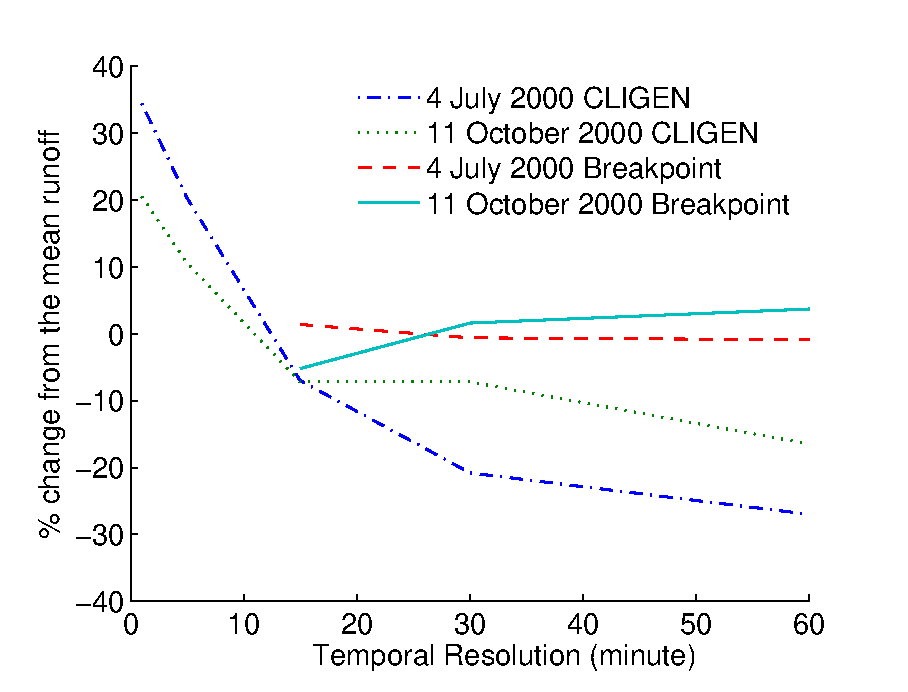
\includegraphics[width=0.5\textwidth]{./img/wepp_runoff_temp_scale}}
    %\qquad
    \subfloat[][Soil
Loss]{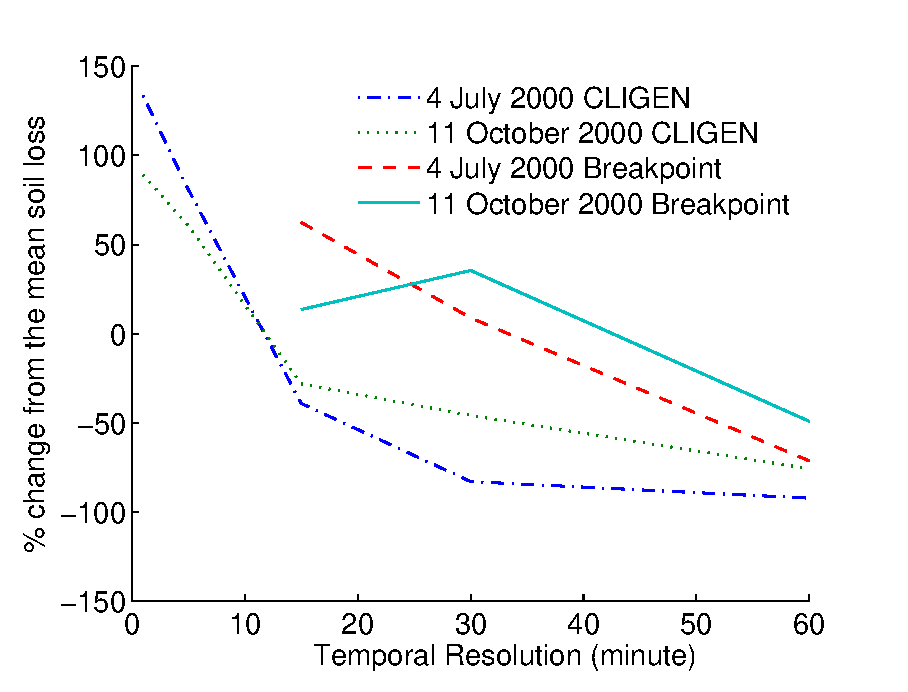
\includegraphics[width=0.5\textwidth]{./img/wepp_sloss_temp_scale}}
  \caption[WEPP runoff and soil loss changes]{The changes of WEPP-simulated
runoff and soil loss from average runoff and soil loss. Note the different scale
of y-axis in (b) Soil Loss.}
  \label{fig:wepp_roff_sloss_temp_scale}
\end{figure}

\begin{figure}[p]
  \centering
    \subfloat[][
Runoff]{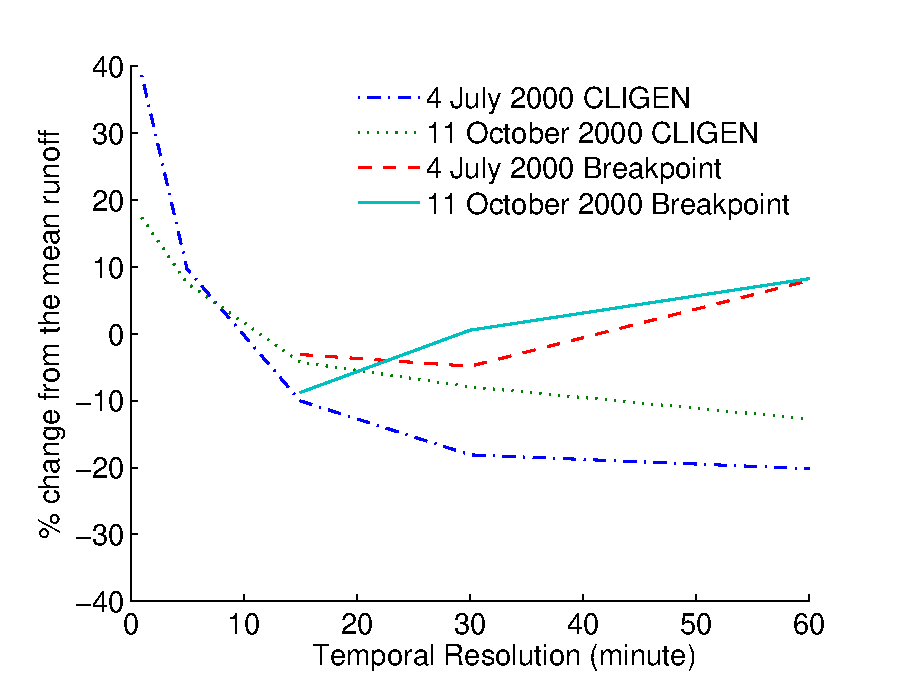
\includegraphics[width=0.5\textwidth]{./img/eurosem_roff_temp_scale}}
    %\qquad
    \subfloat[][Soil
Loss]{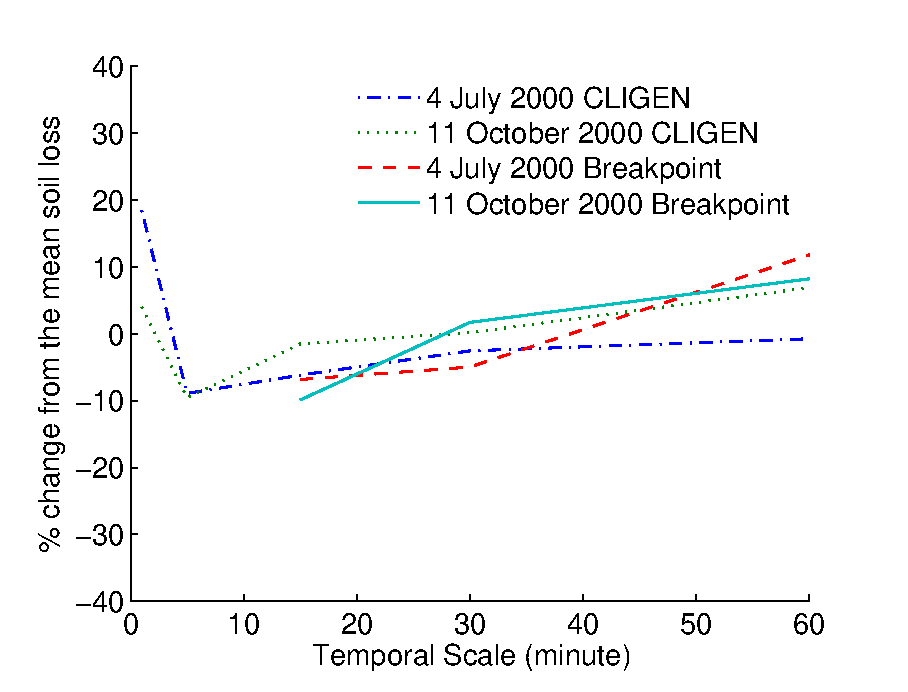
\includegraphics[width=0.5\textwidth]{./img/eurosem_sloss_temp_scale}}
  \caption{The changes of EUROSEM-simulated runoff and soil loss from average
runoff and soil loss}
  \label{fig:eurosem_roff_sloss_temp_scale}
\end{figure}

Changes of temporal resolutions of CLIGEN rainfall data are inversely
proportional
to WEPP-simulated runoff and erosion rates (Figure
\ref{fig:wepp_roff_sloss_temp_scale}). CLIGEN data with higher temporal
resolutions (i.e.\ 1-min and 5-min resolutions) resulted in greater
WEPP-simulated
runoff and erosion rate than CLIGEN data with lower temporal resolutions (30-min
and 60-min resolutions). For breakpoint data, temporal data resolutions have a
varying
effects on WEPP-simulated runoff and erosion rates and do not show clear
correlations with the simulation result (Figure
\ref{fig:wepp_roff_sloss_temp_scale}).

Temporal data resolutions also have certain effects on runoff and erosion rates
simulated by EUROSEM as seen in Figure \ref{fig:eurosem_roff_sloss_temp_scale}.
However, EUROSEM-simulated erosion rates show rather different results from
results of WEPP simulations. Results of EUROSEM simulations for erosion rates
are mostly the opposite from WEPP simulations with some exceptions. Using CLIGEN
data generally resulted in decreasing runoff and increasing soil loss rates as
temporal resolutions increase. This is rather unexpected because decreasing
runoff
rates are normally accompanied by decreasing soil erosion rates. Also, 1-min
CLIGEN data is the only temporal resolution that show increasing soil loss rates
as
well as increasing runoff rates (Figure
\ref{fig:eurosem_roff_sloss_temp_scale}). For breakpoint data, changes of
temporal resolutions resulted in a moderate increasing trend in both runoff and
erosion rates. However, the correlation is rather weak because of the lack of
data points to consider.

\section{Discussion}
\label{sec:TemporalScalesDiscussion}

Although WEPP documents states that 15-min data are to be used
\citep{flanagan1995-weppusersummary}, 15-min data are not always available for
the erosion modelling studies. Thus, the effect of other temporal resolutions
have
been investigated. The results were compared against those of 15-min data and
average values of runoff and soil loss in terms of the rates of changes (\%) to
highlight the relative effects of the changes.

\paragraph{Maximum number of breakpoints} As mentioned previously, breakpoint
data that were prepared for both July and October events with 1-min and 5-min
data could not be used for WEPP and EUROSEM. This was because WEPP have a limit
on the maximum number of breakpoint which is 50 points per day according to the
model document \citep[see][page 10]{flanagan1995-weppusersummary}. This means
that, for a rainfall event that last for a whole day, for example, 30-min data
is the highest resolution we can use for WEPP simulations because there are only
48 (24 hr/0.5 hr) intervals available per day. This prohibits the use of
breakpoint data with temporal resolution higher than 30-min in theory. In
practice, any temporal resolution could be used as long as the total number of
breakpoints does not exceed 50 points.

Testing with WEPP (v2004.7) revealed that up to 100 breakpoints may be used
without a problem. However, when the number of breakpoints exceeds 100
points, WEPP does not recognise the start and end of a rainfall event correctly,
and re-aggregates the rainfall with multiple starting points (i.e.\ 0 minute
point). Thus, the maximum number of breakpoints it can handle should be
increased to at least 1440 points or more to enable the use of 1-min data or
higher temporal data---that is, when daily event is assumed. EUROSEM have the
same limitation which prevent from using more than 100 breakpoints. When tested
with more than 100 breakpoints, EUROSEM simply does not yield any meaningful
output. Also, EUROSEM has a limit on the total number of time increments which
should not be more than 1000 per simulation
\citep{morgan1998-europeansoilerosion}. This may cause more difficulties when a
storm with an extensively long duration is used for detailed simulations.
Therefore, both models need to increase their dimension of breakpoint data array
to meet the need.

\paragraph{WEPP vs EUROSEM} In terms of soil loss rates estimated by two
models, WEPP exhibited greater responses than EUROSEM to the changes of temporal
data resolutions. Although EUROSEM was not as much sensitive as WEPP to the
temporal
resolution of rainfall data, it showed some responses to the temporal resolution
changes.
The biggest change, which was 26.2 \%, in soil erosion estimations was observed
when 1-min CLIGEN data were used (Table
\ref{tab:DifferentTemporalScalesOfRainfallDataOnEUROSEMSoilLoss}).
In comparison to the WEPP's response (i.e.\ 283.2 \%) for the same CLIGEN data,
the change was considerably small (Table
\ref{tab:DifferentTemporalScalesOfRainfallDataOnWEPPSoilLossEstimation}). Even
with breakpoint data, 20.1 \% change for 60-min breakpoint data was the largest
change for EUROSEM (Table
\ref{tab:DifferentTemporalScalesOfRainfallDataOnEUROSEMSoilLoss}). Again, WEPP
estimated 55.2 \% change for the same breakpoint data (Table
\ref{tab:DifferentTemporalScalesOfRainfallDataOnWEPPSoilLossEstimation}).

Moreover, EUROSEM results for CLIGEN data were contradictory to the physical
process of soil erosion. As shown previously, EUROSEM generated increased soil
loss when runoff was decreased (Figure \ref{fig:eurosem_roff_sloss_temp_scale}).

\begin{table}[htbp]
\figureversion{tabular}
\footnotesize
\caption{Summary of detailed EUROSEM outputs estimated with CLIGEN data}
\begin{center}
\begin{tabular}{lrrrrrr}
\toprule
\multicolumn{1}{l}{} & \multicolumn{1}{l}{} & \multicolumn{5}{c}{Temporal
Resolution (min)} \\ \cmidrule{3-7}
\multicolumn{1}{l}{Output} & \multicolumn{1}{c}{Event} & 1 & 5 & 15 & 30 & 60 \\
\midrule
Gross Rill Erosion & 04 July 2000 & 10.4 & 8.8 & 10.3 & 10.7 & 10.9 \\
(t/ha) & 11 October 2000 & 17.5 & 16.9 & 23.4 & 24.1 & 25.6 \\ \midrule
Gross Interrill Erosion & 04 July 2000 & 2.8 & 1.2 & 0.011 & 0.009 & 0.008 \\
(t/ha) & 11 October 2000 & 7 & 4.6 & 0.028 & 0.024 & 0.02 \\ \midrule
Net Erosion & 04 July 2000 & 13 & 10 & 10.3 & 10.7 & 10.9 \\
(t/ha) & 11 October 2000 & 24.7 & 21.5 & 23.4 & 23.8 & 25.4 \\ \midrule
Net Rainfall & 04 July 2000 & 73.9 & 73.9 & 73.9 & 73.9 & 73.9 \\
(mm) & 11 October 2000 & 132.9 & 132.9 & 132.9 & 132.9 & 132.9 \\ \midrule
Rain Duration & 04 July 2000 & 312 & 666 & 798 & 840 & 840 \\
(min) & 11 October 2000 & 444 & 768 & 930 & 1020 & 1080 \\ \midrule
Peak Intensity & 04 July 2000 & 55.9 & 40.5 & 19.7 & 14.7 & 13.5 \\
(mm/h) & 11 October 2000 & 79.4 & 54.6 & 22.8 & 19.5 & 15.7 \\ \midrule
Runoff Duration & 04 July 2000 & 199 & 210 & 336 & 415 & 451 \\
(min) & 11 October 2000 & 433 & 355 & 704 & 656 & 848 \\ \midrule
Peak Runoff Rate & 04 July 2000 & 51.7 & 35.5 & 15.8 & 11.1 & 10.1 \\
(mm/h) & 11 October 2000 & 73.3 & 51.8 & 19.8 & 16.8 & 12.8 \\ \midrule
Time to Peak Runoff & 04 July 2000 & 202 & 389 & 444 & 461 & 473 \\
(min) & 11 October 2000 & 63 & 359 & 459 & 936 & 722 \\ \midrule
Infiltration & 04 July 2000 & 20.2 & 31.9 & 39.5 & 42.5 & 43.4 \\
(mm) & 11 October 2000 & 31.2 & 40 & 50.3 & 52.7 & 57.5 \\ \midrule
Runoff & 04 July 2000 & 53.5 & 42.1 & 34.6 & 31.5 & 30.7 \\
(mm) & 11 October 2000 & 102.1 & 93.6 & 83.3 & 80.1 & 75.9 \\ \bottomrule
\end{tabular}
\end{center}
\label{tab:eurosemscaleresultdetails}
\end{table}

A close examination of EUROSEM model outputs revealed that the estimated amount
of ``Gross Interrill Eroison'' was substantially greater for 1 and 5-min CLIGEN
data than for 15, 30 and 60-min CLIGEN data (Table
\ref{tab:eurosemscaleresultdetails}) while the amount of ``Net Erosion Rate''
was roughly the same. This means that smaller amounts of ``Gross Rill Erosion''
were estimated for 1 and 5-min data resolutions than for the bigger temporal
resolutions.
Thus, it seems that there is a certain change in the way that EUROSEM calculates
rill and interrill erosion rates when the temporal resolution of data changes
from
15-min to 5-min and vise versa.
As reviewed previously in Chapter \ref{sec:PROBLEMINTHECONTEXT} (see page
\pageref{sec:TransportCapacityOfTheFlow}), the model document
indicated that EUROSEM uses separate transport capacity relationships for rill
and interrill flows: \citet{govers1990-45} for rill transport capacity and
\citet{everaert1991-513} for interrill transport capacity. The same is true
for WEPP too as rill and interrill erosion are calculated using separate
erodibility parameters \citep{flanagan1995-usda}. However, in EUROSEM, one seems
to play more important role than the other on overall erosion depending on the
surface condition:

\begin{itemize}
  \item The surface may contain no rills, but have some surface irregularities
    \subitem \textrightarrow\ Interrill erosion is simulated with a high
proportion of the soil surface covered by shallow overland flow.
  \item The surface may be rilled, with interrill flows routed toward the rills
    \subitem \textrightarrow\ both shallow flow between rills and downslope flow
with bigger carrying capacities are simulated.
  \item The surface may be furrowed, or have very dense rills, such that
interrill routing is illogical due to the short distance traversed by interrill
flows
    \subitem \textrightarrow\ ``overbank'' flow is considered. The two areas
(i.e.\ rill and interrill) are connected as surface elevations become equal. The
unified rill profile model can be used.
\end{itemize}

The EUROSEM model document also stated that EUROSEM uses a dynamic approach for
estimating the spatial temporal distribution of runoff and soil loss
\citep{morgan1998-europeansoilerosion}.

Therefore, when temporal resolution of rainfall data changes from 15-min to
5-min,
the slope surface condition, which EUROSEM simulates, seems to shift from the
third condition to the second condition from the list above. Then, EUROSEM
changes its simulation mode so that interrill erosion becomes accounted for.
This explains why the relatively large interrill erosion was estimated for 1 and
5-min resolutions. Thus, it could be suggested that the transition of the
simulation
mode occurs somewhere between 5-min and 15-min of temporal resolutions.

Yet, reasons for the disagreement between runoff and soil loss rate can
not be explained by this ``mode-shifting'' as well as the reduction of net
erosion for 5-min data. An in-depth investigation could be suggested to explain
this finding fully as a follow-up study after this research.

\paragraph{CLIGEN vs Breakpoint data} Rainfall parameters in the CLIGEN
input file were originally calculated from 15-min breakpoint data. CLIGEN then
used this statistical information to simulate continuous long-term daily
rainfall data, which have similar statistical characteristics as the observed
data, or individual storm data could be manually calculated to be in the form of
four unique parameters: rainfall amount, rainfall duration, normalised peak
intensity and normalised time to peak. These four parameters were then used by
WEPP to disaggregate the daily rainfall data into ten breakpoint data using a
double exponential function.

In total, original breakpoint data had gone through two parametrisation
processes effectively. Thus, this procedure of ``parametrisation and
disaggregation'' seems highly inefficient in retaining original rainfall
intensity information, particularly for the event with a long duration and low
intensity which is similar to the event occurred on 11 October 2000. The
rainfall information can be distorted and lost during these data
``parametrisation and disaggregation'' processes.

When the details are lost, it is prone to lead to wrong simulation results. It
is paramount to maintain intensity details such as the number of intensity peaks
that occur during a storm period regardless of frequency in order to study how
these intensity peaks might affect the erosion process. Assuming just one peak
per storm is also a rather crud way of dealing rainfall intensity changes within
a storm.

One reason why WEPP-CLIGEN use such method seems to be because of the ease of
use and data storage for long-term rainfall records. This method---statistically
summarising historical climate data and maintaining it---is a very efficient way
of storing a large amount of rainfall data. One file (i.e.\ CLIGEN input file)
per weather station requires much less space than tipping-bucket data for, say,
10 to 20 years. This however does have a couple of disadvantages:
\begin{enumerate*}
  \item The concept of CLIGEN data is only suitable for convective storms which
do not have many intermittent rainfall phases (no-rain periods) during rainfall.
\medskip
  \item For WEPP to disaggregate CLIGEN data realistically using a double
exponent function, each storm should have one distinctive high rainfall peak.
Such storms are not typical of many parts of the world, and may be seasonally
dependent.
\end{enumerate*}
It is, however, evident that CLIGEN data type make it easier to deal with vast
amounts of data. It also requires considerably less space to store such data.
Also, CLIGEN data are very easy to use with WEPP as it is designed specifically
for this purpose.

If only two extreme ends of the resolution are considered from the result shown
previously in Table
\ref{tab:DifferentTemporalScalesOfRainfallDataOnWEPPSoilLossEstimation} and
\ref{tab:DifferentTemporalScalesOfRainfallDataOnEUROSEMSoilLoss}, for example,
between 1-min and 60-min CLIGEN data, simulated erosion rates with 1-min data
are almost 30 times greater at most than those with 60-min data. This certainly
is problematic as far as the effect of temporal resolutions of rainfall data on
erosion rates is concerned.

Also, when erosion rates estimated with 15-min and
60-min breakpoint data are compared, erosion rates with 15-min data is over 5
times greater at most than those with 60-min data. Again, a greater difference
is observed when erosion rates estimated with CLIGEN data for the same temporal
resolutions are compared. Erosion rates with 15-min CLIGEN data are 7.5 times
greater
at most than those with 60-min CLIGEN data.

Therefore, breakpoint data generally produce smaller changes in erosion rates
when temporal resolutions are changed. This however is not conclusive by any
means
because the responses of two models (i.e.\ WEPP and EUROSEM) are rather
contradictory for both CLIGEN and breakpoint data in terms of their trends of
increases or decreases.

\paragraph{Data aggregation and rainfall intensity} The intensity information
of rainfall data is heavily dependent on how they are aggregated. When rainfall
data such as tipping-bucket data are aggregated into certain time steps, they
are usually stored in a digitized data format. It means the averaged rainfall
intensity is dependent on the start time as well as time-steps which is temporal
resolutions. Time-steps and start time are important as the rainfall intensity
is
averaged over the given time-steps and start point when they are archived. This
method, however, unintentionally discards rainfall intensity information by
averaging rainfall peaks over the given time step.

The effect of discarding rainfall intensity information has been clearly shown
when both rainfall events---i.e.\ 4 July 2000 and 11 October 2000---were
aggregated into varying time steps. Distinctive high intensity peaks in 1-min
data (Figures \ref{fig:dr_storm-a} and \ref{fig:pl_storm-a}) was no more visible
because intensities were averaged out over the longer time-steps (cf. Figures
\ref{fig:dr_storm-e} and \ref{fig:pl_storm-e}).

\paragraph{Effect of temporal resolution changes} Two effects can be noted when
temporal resolution increases. One is that it lowers of the actual instantaneous
peak
intensity and average intensity of rainfall storms. The other is that it
changes the location of peak intensities during storm durations.

Lowering the average intensity means a reduced average power of erodibility
of the rain. Also, lowering the peak intensity means a reduced instantaneous
peak power of erodibility of the the rain. These reductions in erodibilities may
be a significant reason for the underestimation of the runoff and soil loss
generations. Equally, the opposite can be expected when temporal resolution
decreases. Some of these responses are observed in this chapter (see Figures
\ref{fig:wepp_roff_sloss_temp_scale} and
\ref{fig:eurosem_roff_sloss_temp_scale}).

Shifting the location of the peak rainfall intensity can occur when temporal
resolutions are changed regardless of increase or decrease. Also, the placement
of
the peak intensity do not seem to be related to the direction of changes (see
Table \ref{tab:CLIGENWEPPInputFileParameters} and Figures
\ref{fig:dr_storm}--\ref{fig:pl_storm}). However, When the location of the peak
intensity changes, it too changes rainfall shapes (or patterns) which may be
closely related to the timing of the runoff generations and amount of the runoff
(This is further investigated and discussed later in Chapter
\ref{sec:EFFECTSOFRAINFALLINTENSITYCHANGESONSOILEROSION}.). Thus, changes in
temporal resolutions of rainfall data affect the shape of rainfall storm.

All these changes---lowering of intensities and shifting the location of peak
intensities---will of course occur simultaneously when the temporal resolution
of
rainfall data is altered. Thus, what we observed in this chapter may well be the
end product from compound effects of these two changes. Effects of lowering of
intensities and shifting the location of peak intensities on runoff and
soil loss rates therefore need to be investigated separately to be understood
further.

\paragraph{Within-Storm Intensity Variation (WSIV)} The variation of rainfall
intensities within a storm could be termed as Within-Storm Intensity Variation
(WSIV) for convenience. WSIV may include the magnitude and number of peak
intensities and average intensity of a storm. As suggested previously, WSIV is
related to temporal resolutions of rainfall data as well as types of storms
(e.g.
convective and frontal). WSIV changes when rainfall intensities are decreased
(or increased) by increasing (or decreasing) temporal resolutions of rainfall
data.

\citet{wainwright2002-1271} carried out numerical experiments to test if
temporal variability of rainfall intensity during a storm can cause the decrease
in runoff coefficients with increasing slop length. They found that variability
of temporal resolution in rainfall is a significant factor in controlling the
resolution-dependency of runoff coefficients. Also, overland-flow models which
use
mean rainfall intensities may notably under-predict the runoff.
High rainfall intensity is closely related to high rainfall kinetic energy,
which controls runoff generation and soil loss. Yet the way of archiving and
aggregating long term rainfall data into a manageable data format may let
important rainfall intensity details to be missed out as shown in this chapter.

\citet{boardman1987-36} also pointed out that
short period high intensities probably important for soil erosion processes.
However, short duration rainfall intensities are subject to a large uncertainty,
especially when they are produced during extreme convective rainfall events
\citep{garcia2001-675}. In the study by \citet{garcia2001-675}, 408 rainfall
events have been statistically analysed for the period 1925-1992 in Alicante,
Spain. Maximum intensities for durations ranging from 2 minutes up to 240
minutes were extracted from the series \citep{garcia2001-675}. Considerable
differences are found in the behaviour of the empirical functions for short
durations (t < 10 minutes) \citep{garcia2001-675}. The energy of individual
storms could only be predicted with limited accuracy because of natural
variations in rainfall characteristics \citep{vandijk2002-1}.

% For future soil erosion studies, one needs to know about future rainfall
% intensity. But without high resolution rainfall data, one may predict future
% soil erosion with a large error as shown by this investigation.  Even with
% 15-min data it is possible to get as much as about 3 times less soil erosion
% estimation compared to 1-min data. This may pose a problem when using large
% scaled GCM or RCM rainfall data directly for soil erosion. It is relatively
% difficult to predict rainfall intensity changes with good reliability even with
% a climate model.

Thus, high temporal resolution data are needed in order to describe WSIVs of
storms realistically. High temporal resolution data can provide great details of
WSIVs including high instantaneous intensity peaks. However, high resolution
data even as sub-hourly data are very rarely available.
As \citet{allott2002-73} pointed out, rainfall data with high resolutions permit
a more detailed assessment of the storm structure and evolution of localised
intense storms, but storms are rarely stored by sub-hourly.

Even though storms are often originally recorded as sub-hourly data by
tipping-bucket gauges, the original records are rarely kept as they are.
Instead, they are usually aggregated into hourly or daily data for data storage.
Thus, only hourly or daily data are available in many cases.
Therefore, a little is ever known about the storm structure, evolution and, of
course, WSIVs. With hourly (or more generally daily) data, the detail of
actual rainfall intensity can not be obtained. This has been shown
previously by comparing Figure \ref{fig:pl_storm-a} and Figure
\ref{fig:pl_storm-e}, for example. The differences in WSIVs between hourly data
and 1-min data may have been particularly responsible for the great
dissimilarities in runoff and soil loss rates between two temporal resolutions.

Therefore, it is evident that temporal resolutions of rainfall data play a
crucial role in runoff and soil loss modelling. Changes of temporal resolutions
affect the amount of details on WSIVs which, in turn, affect runoff and soil
loss estimations.
Sub-hourly data hold more details of WSIVs than hourly data. Thus, it would be
logical to choose sub-hourly data over hourly data (i.e.\ 60-min resolution) for
erosion modelling. Also, because breakpoint data are less affected by the
changes of temporal resolutions than CLIGEN data, breakpoint data can be
preferred to CLIGEN data. In addition, breakpoint data maintains the detail of
WSIV better.

Among the investigated sub-hourly resolutions, 1-min and 5-min resolutions of
breakpoint data cannot be used, however, because WEPP and EUROSEM have the
limited number of rainfall data points they can handle. Now there are only two
choices left: 15-min and 30-min breakpoint data.
There could be other sub-hourly resolutions available, for example, 10-min,
20-min and so on. However, these other sub-hourly resolutions were not
considered here because investigations were only carried out with the ones used
in this chapter: 1, 5, 15, 30 and 60-min. Therefore, within the temporal
resolutions investigated in this chapter, 15-min data were chosen. This temporal
resolution will be used for the subsequent analyses in this research because
they have greater details of WSIVs than 30-min data. Moreover, WEPP and EUROSEM
can easily use 15-min breakpoint data.

It is also recognised that different ways of expressing rainfall intensity have
the tenancy of desirability for erosion modelling. This is summarised in Table
\ref{tab:DesirabilityOfDifferentWaysOfExpressingRainfallIntensity}.

\begin{table}[htbp]
  \small
  \centering
      \caption{Desirability of different ways of expressing rainfall intensity}
  \label{tab:DesirabilityOfDifferentWaysOfExpressingRainfallIntensity}
    \begin{tabular}{ccl}
    \toprule
    Similarity to Reality & Desirability & Method of Rainfall Data
Representation\\
    \midrule
    Dissimilar & Most & Amount, Duration, Time-to-Peak \& Peak Intensity\\
    $\uparrow$ & $\uparrow$ &  Breakpoint Data without `no rainfall periods'\\
    $\downarrow$ & $\downarrow$ &  Breakpoint Data with `no rainfall periods'\\
    Similar & Least & Tipping Bucket Data\\
    \bottomrule
    \end{tabular}
\end{table}

Even though breakpoint data hold more information and are closer to real
rainfall than CLIGEN data, it still has some problems. The temporal resolution
of breakpoint data limits their closeness to real rainfall since rainfall
intensity is averaged between starting and ending time of breakpoints.

Lastly, it is important to note again that a erosion model should be able
to take high resolution data such as 1-min breakpoint data. Once this
limitation is resolved, other sub-hourly data resolutions may also become
available for the similar investigation conducted in this chapter. This, in
turn, extend the findings presented in this research.

\section{Conclusion}
\label{sec:TemporalScalesConclusion}

This set of investigations evidently showed that temporal resolution of rainfall
data have certain impacts on runoff and soil loss estimations. However, it could
not answer if rainfall data with a high resolution always give better simulation
results than rainfall data with a low resolution. This is because there are
no measured runoff and soil loss rates to compare. Despite the absence of the
measured data to be compared with, this chapter identifies the close
relationship between temporal resolutions and WSIVs of rainfall data. When
temporal resolutions of rainfall data increase (or decrease), rainfall
intensities are decreased (or increased). WSIVs are also changed when rainfall
intensities of storms change.

If there are no available high resolution data but only low resolution
data (e.g. 60-min data), we will never know what the intensity was like
during those 60 minutes because the disaggregation of rainfall data is no
plausible. Also, simulation results can be up to about 30 times different from
the ``original results'' if these low resolution data are used. This magnitude
is so great that it might mean from almost no erosion to disastrous events.

%What temporal scaled rainfall data should I suppose to use? and why?
%What can we expect to happen if we use other temporal data?
In this chapter, the following was found:
\begin{itemize}
  \item Temporal resolutions of rainfall data affect Within-Storm Intensity
Variations (WSIVs)
  \item Temporal resolutions of rainfall data are closely related to the
estimated
results of runoff and soil loss
  \item In terms of soil loss, WEPP is more sensitive to the change of temporal
data resolutions than EUROSEM
  \item Erosion estimations with CLIGEN data are more affected by the change of
temporal resolutions than those with breakpoint data
  \item Breakpoint data are preferred to CLIGEN data as far as investigations
on effects of rainfall intensity on erosion are concerned
  \item For the subsequent analyses of this research, 15-min breakpoint rainfall
data are chosen
\end{itemize}


As stated previously, this chapter is followed by a further investigation which
aims to answer the research question: `\textit{What is the consequence of
removing the no-rain periods within a storm duration?}'. The removal of no-rain
periods---that is later termed as Within-Storm Gaps (WSGs)---is required during
CLIGEN data preparation processes. However, it raises a concern that the removal
of WSGs may lead to a loss of rainfall intensity information. More worryingly,
a distortion of rainfall patterns and feeding this wrong information into soil
erosion models could also occur. In the next chapter, therefore, effects of
WSGs on soil erosion estimations are investigated.


%******put B2B test here (intensity burst test)????
%\nolinenumbers

%%%%%%%%%%%%%%%%%%%%%%%%%%%%%%%%%%%%%%%%%%%%%%%%%%%%%%%%%%%%%%%%%%%%%%%%%%%%
%\section{Discussion on CLIGEN versus Breakpoint Data}
%\label{sec:tpipbpIntroduction}
%
%When rainfall data are used for erosion modelling, two data types are
%available---CLIGEN and breakpoint data. In this section, these two rainfall
%data types are compared in terms of runoff and soil loss generations using
%WEPP and EUROSEM.
%
%This section aims to determine which rainfall data input method is more
%desirable for the subsequent investigations of the effect of rainfall
%intensity on soil erosion.
%
%The storm observed on 4 July 2000 is a typical summer rainfall event in the
%UK. It has a relatively short duration with a rapid rainfall intensity
%change during the storm period. The storm which fell on 11 October 2000
%with a longer duration can typically be observed in the British autumn
%periods. It sometimes lasts over few days with a gradual rainfall intensity
%change, often followed by severe floods.
%
%Original peak intensity of the storm is unchanged. Only duration is changed
%because of removal of no-rain periods from the total storm duration.
%
%This may be a problem as it clearly does not use the same data directly.
%However, as WEPP also uses the same 10 breakpoint data disaggregated from
%CLIGEN data, there should not be any differences in the values used for
%calculating runoff and soil loss. Moreover, this test is to find out what
%rainfall intensity information we might miss out by using one data form
%instead of another, and the consequence of using such data. This means that
%the efficiency of each data form is not the main interest here although it
%might be related to the actual outcomes of this test.
%
%As there is no observed runoff and soil loss data, it may be difficult to
%prove which data type gives better (or realistic) erosion results. Thus,
%each data type is compared in terms of characteristic differences. %pros
%and cons, closeness to real rainfall patterns, retaining intensity
%information can be discussed here.
%Does it have no artefacts in simulating erosion? (This is as mentioned
%difficult to find because of no measurement) Does it really matter for
%erosion estimation? rainfall duration? Is the differences in the result
%obvious? Did the result really show clearly breakpoint data type is
%superior and preferred type over the CLIGEN data type? Is the result true
%for both storm? (very unlikely!)


%\subsection{Conclusion}
%\label{sec:tpipbpConclusion}

%Which type of the data provide more realistic information on rainfall
%intensity?

%\section{Suggestions for Further Investigations}
%\label{sec:FurtherInvestigationSuggestion}
%%%%%%%%%%%%%%
%You need to think about the order of chapters in the next part.
%temporal resolution, intensity patterns, and gaps

%Use Tony's work and rillgrow in intensity pattern. this then give you the
%reason for using rillgrow result as reference in gap test.
%
%Ask all the questions that are going to be addressed in the next part.
%%%%%%%%%%%%%%
%This chapter is followed by a number of further research questions.

%One is that, if we choose to use breakpoint data over CLIGEN data, what is
%the appropriate data resolution to use? Any sub-daily data are going to be good
%enough? Moreover, CLIGEN rainfall parameters (precipitation amount  (mm),
%$R$, storm duration (hour), $D$, time to peak as a fraction of the storm
%duration, $t_p$, and the ratio of peak  intensity over average intensity,
%$i_p$) are calculated originally from 15-min rainfall data. This, however,
%overlooks the variations of rainfall intensity within 15 minutes.
%Therefore, it is suggested to test effects of different temporal resolution of
%data on soil erosion.

%The second question is `What are the consequence of removing the no-rain
%periods within a storm in order to estimate CLIGEN data?'. Is this going to
%be ok to just ignore these intermittent rainfall pattern and consider them
%as a continuous rainfall? These questions can be answered by continuous and
%discontinuous storm test.

%This continuous and discontinuous storm test may seem very similar to the
%previous test discussed just now. But, it is not!

%Let's be clear about this. comparison done between BP and CLIGEN data is to
%find which type of data representation is better than the other for erosion
%simulation. So, two different types of storms are chosen for the test.

%The suggested test (second one) raises an issue about the no-rain periods
%that is removed during data preparation, which in turn, may lead to a loss
%of rainfall intensity information. more worryingly distorting rainfall
%intensity information and feed this wrong data into soil erosion models.
%So, only one storm that has few recognizable intermittent gaps within the
%storm duration is subjectively selected and tested.
